\section{Define the estimand before the leaderboard}\label{sec:C26:estimand}
Let $D$ be a task distribution, $S$ a system configuration, $B$ a resource envelope, and $Y$ a declared outcome. The primary estimand can be written $\mu(S,B,D)=\mathbb E_{x\sim D}[Y(S,B,x)]$. Formally, $D$ is a probability measure on an eligible task space $\mathcal X$, and $Y$ is integrable under the joint task and execution randomness; a normalized success outcome has range $[0,1]$. Every symbol carries a substantive choice. Tasks can be sampled by repository, user, domain, or time. Resources can constrain money, elapsed time, attempts, or tool access. Outcomes can measure final correctness, constraints, latency, or utility. A numerical ranking is uninterpretable without these choices.

Micro- and macro-averages answer different questions. A micro-average weights each task equally, so a large task family dominates. A macro-average gives equal weight to families, potentially giving a small noisy group disproportionate influence. Neither is universally correct. Report the weighting rule and family-level results, and avoid changing weights after seeing which system benefits. Where a deployment distribution is known, a workload-weighted estimate can be relevant, but its sampling uncertainty and drift remain material.

The system boundary should include model checkpoint or service identity, prompt and harness revision, tools, memory policy, evaluator, and environment. A benchmark score obtained with a newer parser or different hidden-test version is a different observation even if the headline labels are unchanged. Closed service revisions may be unavailable; then the result is a dated service evaluation rather than a fully reproducible checkpoint comparison.

The foundational 2022 HELM framework emphasizes multidimensional evaluation across scenarios and metrics~\cite{liang2022helm}. For agents, this perspective extends naturally to permission compliance, state consistency, external effects, and recovery. A system can improve success while worsening cost or security. A scalar utility can summarize those tradeoffs only after the weights and acceptable constraints are justified. It should not conceal a hard safety or authorization requirement inside a favorable average.

The practical first step is an evaluation contract that names the target population, eligibility rules, unit of analysis, allowed information, resource limits, stopping conditions, and outcome definitions. This contract supports later auditing because it makes deviations visible. It also prevents an experiment from drifting into a different question when difficult cases or infrastructure failures appear.


% SCIENTIFIC_FIGURE_C26
Figure~\ref{fig:C26:overview} contrasts selection feedback with the one-way transfer of a frozen artifact to sealed evaluation.
\begin{figure}[!htbp]
\centering
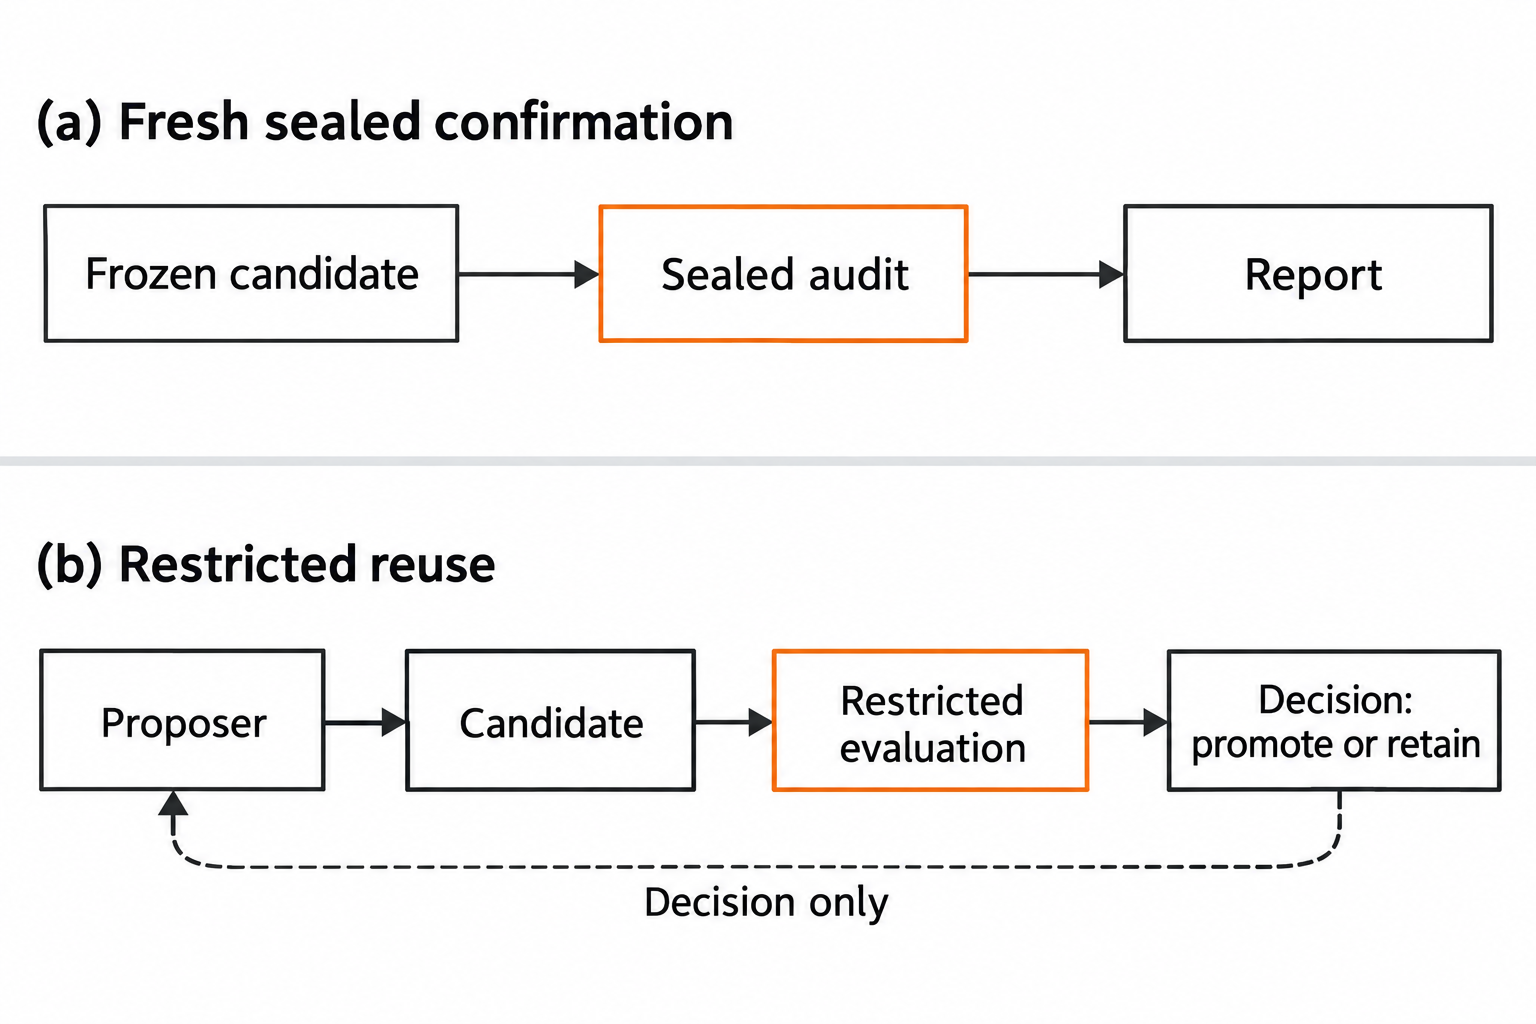
\includegraphics[width=\linewidth]{book/figures/assets/F26review.png}
\caption{Two evaluation protocols with distinct feedback boundaries. Fresh sealed confirmation returns a report outside selection. Restricted reuse exposes only promotion decisions to the proposer; validity additionally requires the source protocol's initial evaluation independence and history-wide error allocation. The feedback restriction alone is not an error-control proof. No experimental outcomes are depicted.}
\label{fig:C26:overview}
\end{figure}
